%% V1.0
%% by Gabriel Garcia, gabrcg@gmail.com
%% This is a template for Udacity projects using IEEEtran.cls

%% Be Udacious!

\documentclass[10pt,journal,compsoc]{IEEEtran}

\usepackage[pdftex]{graphicx}    
\usepackage{enumitem, mathtools, amssymb}
\usepackage[colorlinks=true, urlcolor=blue, linkcolor=blue]{hyperref}

\hyphenation{o-do-me-try pa-ra-me-ter}
\raggedbottom
\begin{document}

\title{Robot Localization -- Where Am I?}
\author{Stephan Hohne}

\markboth{Project 6, Robotics Software Engineer Nanodegree Program, Udacity}%
{}
\IEEEtitleabstractindextext{%

\begin{abstract}
Two models of mobile robots are created with URDF in a simulated Gazebo environment. Their task is to perform localization and path planning within a given 2D map. They have to reach a given goal location with the highest precision possible in a reasonable amount of time. The robots are equipped with a camera and a laser scanner. The ROS navigation stack is applied to process the sensor data and move the robot models. The adaptive Monte Carlo localization ROS package is applied to perform probabilistic localization with a particle filter. The parameter space of both packages is explored in order to optimize the navigation performance of the robot models.
\end{abstract}

\begin{IEEEkeywords}
Kalman Filters, Monte Carlo Localization.
\end{IEEEkeywords}}

\maketitle
\IEEEdisplaynontitleabstractindextext
\IEEEpeerreviewmaketitle
\section{Introduction}
\label{sec:introduction}
\IEEEPARstart{T}{he} task of localization is to determine the pose of a robot within a mapped environment using sensor measurements and control inputs. In the real world, sensor and control data are noisy and inaccurate. Velocity commands may not be executed perfectly due to slip between wheels and underground. External forces like wind or water may dislocate the robot in a way that the sensors can't cope with. As a result, the robot can not rely on the validity of the information about its current state in the environment.

The problem of localization relative to a given map can be split into three types, see section $9.1$ in \cite{principles_of_robot_motion}. In the position tracking problem, the initial pose of the robot is given, and the robot can associate a measurement like a camera image with the corresponding feature on the map. In the global localization problem, the initial pose is unknown, and the robot can not uniquely match an observation with one of the features on the map. The relocalization problem is the most complex one. It covers situations where the robot forms a false belief about its current state, because the measurement data do not match the current state of the robot.

The methods of probabilistic localization are designed to solve these types of problems. Among the solutions are Kalman filter and particle filter implementations like Monte Carlo localization \cite{principles_of_robot_motion}, \cite{probabilistic_robotics}. In order to accommodate for uncertainty, these methods formulate the problem in terms of probability distributions. The current state of the system is represented by a belief, which is a probability distribution over possible states. The task of the algorithm is to give an estimate of the current state given the previous state and sensor measurements. This is accomplished by filtering for the belief that represents the most likely state estimate.

Formally, the robot and its environment are formulated in terms of a dynamic stochastic system. Kalman and particle filters implement this system in different ways, see sections $8.2$ and $9.1$ in \cite{principles_of_robot_motion} The Kalman method can solve the position tracking problem, whereas particle filters can handle the global and relocalization problems as well. The specifics are discussed further in section \ref{sec:background}. 

In this project, two models of mobile robots are designed. In a Gazebo simulated environment, their task is to evaluate camera, laser scan, and odometry data to navigate across the given 2D map and reach the given goal location. For both models, the ROS navigation stack is set up following \cite{ros_wiki_nav_stack}. The Adaptive Monte Carlo Localization (AMCL) algorithm is applied to solve the position tracking problem. The configuration of the AMCL and move base packages is studied and optimized for navigation performance of each robot model. 

This report is organized as follows. In section \ref{sec:background}, the Kalman and particle filter algorithms are described and compared. In section \ref{sec:simulations_robot_models}, the design of two robot models is described. In section \ref{sec:background_navigation_stack}, the configuration of the ROS navigation stack is detailed. In section \ref{sec:simulations_parameter_tuning}, the experiments for exploring the navigation stack parameter space are described. The results of the parameter tuning experiments and the robot model test runs are reported in section \ref{sec:results}. The navigation performance of the robot models is discussed in section \ref{sec:discussion}. Concluding remarks and an outlook to future work are given in section \ref{sec:future_work}. 

\section{Background: Localization Algorithms}
\label{sec:background}
In the real world, robotic systems are faced with noisy sensor measurements and odometry data. Yet in most application scenarios it is necessary to maintain an accurate estimate of the current pose of the robot. Therefore it is important to tackle the challenge of localization with a probabilistic framework. This section starts with a discussion of Bayesian methods applied to localization, following section $9.1$ in \cite{principles_of_robot_motion}. It continues introducing the Kalman filter and particle filter algorithms (following \cite{principles_of_robot_motion}, \cite{monte_carlo_for_mobile_robots}) and closes with a comparison of these algorithms. 

Probabilistic localization methods estimate a robots pose relative to a given map in the presence of uncertainty. The robot and its environment are represented by a dynamic stochastic system,. The continuously varying robot state is sampled at discrete, evenly spaced time intervals. The current state of the system at time step $t$ is represented by the robot state $x_t \in \mathbb{X}$, where $\mathbb{X}$ is the state space of the robot, the measurements $y_t$ and controls $u_t$. Examples for measurement data $y_t$ are obstacle distances derived from camera images or laser range scans. Examples for control inputs $u_t$ are velocity commands and odometry data.

To formulate the transition of the system from one time step $t-1$ to the next step $t$, this dynamical system is characterized by the motion model and the observation model. The motion model uses control input data $u_{t-1}$ to predict the change of state in the environment when going from $t-1$ to $t$. It is defined as the probability of the current state conditioned on the previous state and the previous control inputs,
\begin{equation}
\label{eqn:motion_model}
P \left( x_t \vert u_{t-1}, x_{t-1} \right) \, .
\end{equation}
When expressed as a transition probability, \ref{eqn:motion_model} represents the probability that the control command $u_{t-1}$ carries the system from state $x_{t-1}$ to $x_t$. The observation model, also called sensor or measurement model, specifies the likelihood of taking the measurement $y_t$ when the system is in state $x_t$. It is defined as the conditional probability of the measurement $y_t$ given the state $x_t$, 
\begin{equation}
\label{eqn:observation_model}
P \left( y_t \vert x_t \right) \, .
\end{equation} 

Given a probability distribution for the current state, the control inputs, the measurements, the motion model, and the observation model, probabilistic algorithms calculate an estimate for the new state in a two step process. In the prediction step, the current state distribution is forward propagated using the controls and motion model. In the update step, this prediction is corrected by comparing it to the sensor output obtained using the observation model. This second step of the estimation process can be interpreted as a filter for the best guess estimate of the new state. 

One specific probabilistic localization method is Bayesian filtering, where the state estimate is represented by the conditional probability distribution 
\begin{equation}
\label{eq:posterior}
P\left( x_t \vert u_{0:t-1}, y_{1:t}\right) \quad \mathrm{posterior}
\end{equation}
over the state space given the sensor measurements $y_{1:t}$ up to the current step and the control input $u_{0:t-1}$ up to the previous step. The task is to determine this posterior state estimate given the prior state estimate 
\begin{equation}
\label{eqn:prior}
P\left( x_{t-1} \vert u_{0:t-2}, y_{1:t-1}\right) \quad \mathrm{prior} \, .
\end{equation}
This is accomplished by the Bayesian formula. It describes how to update the most recent estimate, the prior, using the sensory input and the motion model, to obtain the new state estimate, the posterior. The Bayesian formula can be written down informally as
\begin{equation}
\label{eqn:bayesian_formula}
\mathrm{posterior}  =  \eta_t \mathcal{O}_t \, \mathrm{Sum}_{x_{t-1}} \left( \mathcal{M}_t \times \mathrm{prior}\right) \, .
\end{equation}
The summation is over the previous states. It is a sum in discrete state spaces, or an integral in continuous state spaces. The transition probabilities $\mathcal{O}_t \coloneqq P \left( y_t \vert x_t \right)$ are determined by the observation model and $\mathcal{M}_t \coloneqq P \left( x_t \vert u_{t-1}, x_{t-1} \right)$ are determined by the motion model. The normalization constant $\eta_t$ ensures that the posterior distribution sums up to $1$.

The Bayesian formula \ref{eqn:bayesian_formula} encompasses both the prediction and the update step of the estimation algorithm described above. The Kalman and the particle filter implementations realize the observation model \ref{eqn:observation_model}, the motion model \ref{eqn:motion_model}, and the computation of the posterior belief distribution \ref{eq:posterior} in different ways.

\subsection{Kalman Filters}
The linear Kalman filter assumes that the motion model \ref{eqn:motion_model} and measurement model \ref{eqn:observation_model} are linear functions of their arguments, and that the state space can be modeled by a unimodal Gaussian distribution. The state estimate at time $t$ is expressed as a Gaussian $\mathcal{N}\left(\mu_t , \Sigma_t \right)$ with mean $\mu_t$ and covariance $\Sigma_t$. The motion and measurement models are represented by linear transformation matrices.\footnote{For instance, in the sensor model equation $y_t  = H_t x_t + w_t$, the measurement $y_t$ is assumed to be a linear in $x_t$, with the transformation matrix $H_t$ and an added Gaussian noise term $w_t$.} The dynamic system is then defined by prediction and update equations for the mean and covariance. The full equations can be found in section $8.2.5$ in \cite{principles_of_robot_motion}.

Starting from the given initial belief, the algorithm iterates between state predictions and measurement updates. First, the prediction equation is applied to forward propagate the prior belief. In the update step, the predicted belief is corrected by the measurement data, taking into account the relationship between the accuracy of the predicted belief and the measurement noise. The continuous iteration of the two steps keeps track of the current state.

While linear Kalman filters are fast and easy to implement, their range of application is very limited, since in practice most robotic systems are nonlinear, with the motion and observation model represented by differentiable functions.\footnote{For instance, the sensor model equation $y_t = h\left(x_t, t \right) + w_t$ with the differentiable function $h$.} The Extended Kalman Filter (EKF) handles nonlinear systems by linearizing the prediction equation around the current estimate and the update equation around the current prediction. The differentiable functions for the motion and observation model are approximated by their Jacobians. The full EKF equations can be found in section $8.3$ in \cite{principles_of_robot_motion}.

\subsection{Particle Filters}
Particle filters are a more general approach to localization than the Kalman filter, they allow for arbitrary distributions for sensor noise, observation model, and motion model. Generic probability distributions replace the dynamic equations.

Particle filters represent a belief distribution by a finite set of samples randomly drawn from it. Each sample $(x, w)$ consists of a state vector $x \in \mathbb{X}$ and an importance weight $w \in [0,1]$. Such a sample, also called particle, can be interpreted as a hypothesis of the robot state and its likelihood. 

Particle filters can be initialized with an arbitrary distribution, for instance, a uniform distribution with equal importance weights when the initial pose of the robot is unknown. The algorithm iterates in the familiar two step process of prediction and update. In the prediction step, the motion model \ref{eqn:motion_model} and control input are used to forward propagate each particle in the sample set, and random odometry noise is added to each particle. In the update step, the sensor input and observation model \ref{eqn:observation_model} are used to calculate a new corrected particle distribution. The weight of each particle is computed as the likelihood of the measurement, given the system is in the predicted state. Then, the resampling procedure is applied. A new collection of samples is drawn with replacement from the current set of particles. The probability of selecting a specific particle is proportional to its normalized weight. This ensures that the new particle set is in accord with the weight distribution. The resulting sample set represents the posterior belief of the new robot state.

The adaptive Monte Carlo localization algorithm applied in this project is also capable of handling the relocalization problem \cite{probabilistic_robotics}, \cite{ros_wiki_amcl}. AMCL keeps track of the measurement likelihood. When the observation becomes unlikely given the current state, the resampling process is modified by introducing random poses into the sample. This modification enables the particle cloud to refresh, and the robot can relocate. The corresponding AMCL configuration is discussed in section \ref{sec:discussion}.

\subsection{Comparison}
Kalman filters can be implemented efficiently in order to use only little compute resources. They work well in high-dimensional state spaces and can provide accurate estimates. Since Kalman filters are limited to unimodal Gaussian distributions for representing belief, they can only be applied to systems with known data association. They also rely on an accurate initial belief. Therefore, Kalman filters can only solve the position tracking problem. Linear Kalman filters can be applied to linear systems. EKF can be applied to systems where the linear approximation is valid.

Kalman filters can be applied in sensor fusion systems, where measurements from multiple sensor types are combined to improve accuracy. They are also of advantage when compute resources are limited, like a home robot running Raspberry Pi. They might also be used in applications where a fast estimation is needed, as data is collected.

Particle filters put fewer restrictions on the observation model, the motion model, and the system dynamics. Therefore, they can be applied to a much wider range of nonlinear robotic systems. Particle filters do not rely on a given initial belief. They allow for multimodal distributions as state estimates, whereby they can handle ambiguity in the data association. Therefore, they can solve all three types of localization problem stated above, see section \ref{sec:introduction}.

An example of a real world robot applying Monte Carlo localization is the MINERVA robot, see chapter 5 in \cite{monte_carlo_for_mobile_robots}. In this project, particle filters are applied when using the AMCL package.

\section{Simulations: Robot Models}
\label{sec:simulations_robot_models}
In this project, two different robot models are studied. Both robots are laid out as mobile rovers that can drive differentially on a 2D plane. Both designs can turn in place, but are non-holonomic. They can not go sideways, so no strafing velocity commands can be issued. Both robot models are specified in XML using the Universal Robotic Description Format (URDF). The code for each model is bundled as a separate ROS package, \href{https://github.com/S2H-Mobile/RoboND-Localization-Project/tree/master/udacity_bot}{\texttt{udacity\_bot}} and \href{https://github.com/S2H-Mobile/RoboND-Localization-Project/tree/master/rover}{\texttt{rover}}, respectively.

The benchmark model is the \texttt{udacity\_bot}. It is designed as a basic mobile rover with a rectangular footprint and a box-shaped chassis. There are two differentially driven wheels on the left and right side of the chassis. Two caster wheels located front center and back center below the chassis stabilize the robot while allowing for in-place rotation. A Hokuyo laser is mounted on the top of the chassis in the front center. A forward-looking camera is mounted on the front side of the chassis. The reference model is depicted in figure \ref{fig:udacity_bot}.
\begin{figure}[htpb]
      \centering
      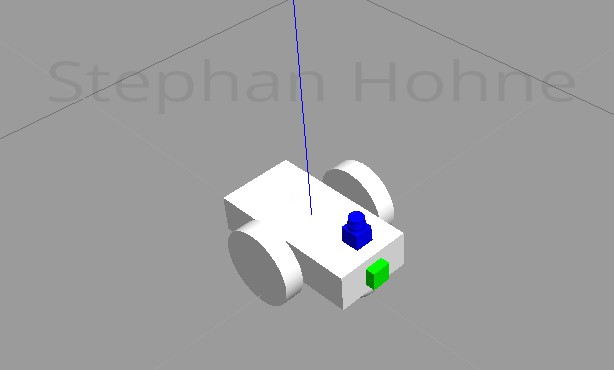
\includegraphics[width=\linewidth]{images/udacity_bot_gazebo_signed.PNG}
      \caption{The reference model \texttt{udacity\_bot} in Gazebo.}
      \label{fig:udacity_bot}
\end{figure}

The custom model is the \texttt{rover}. Its design is based on \texttt{udacity\_bot} with a series of modifications. The custom design was developed in three iterations. In the first iteration, a traditional car layout was used, four wheels on a rectangular chassis, see image \ref{fig:rover_1_design}. With this layout, the rover was not able to turn in place, which hindered recovery behavior, see image \ref{fig:rover_1_stuck}.
\begin{figure}[thpb]
      \centering
      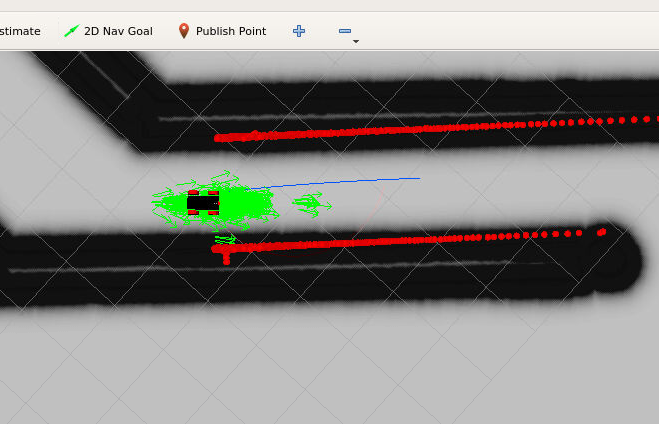
\includegraphics[width=\columnwidth]{images/rover_version_1_1_small.png}
      \caption{First version of custom rover with four wheel design in RViz. Screenshot in RViz with global cost map in background.}
      \label{fig:rover_1_design}
\end{figure}
\begin{figure}[thpb]
      \centering
      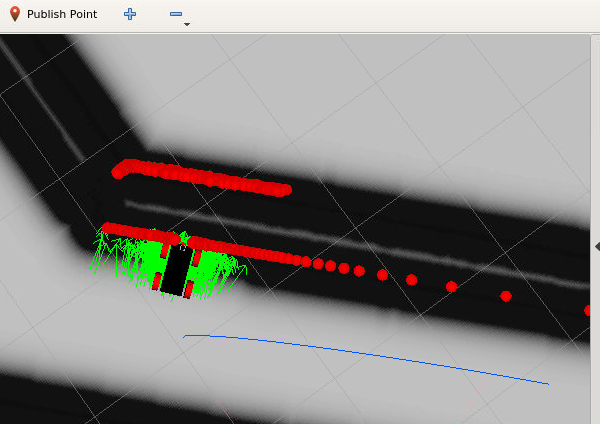
\includegraphics[width=\columnwidth]{images/rover_version_1_5_small.png}
      \caption{First version of custom rover got stuck. Screenshot in RViz with global cost map in background.}
      \label{fig:rover_1_stuck}
\end{figure}

In the second iteration, a three-wheel layout on a box-shaped chassis was used, with two front wheels and a caster in the back center, see image \ref{fig:rover_2_design}. This version was able to rotate in place slowly, yet there was a high risk of toppling over while turning in place close to obstacles, see image \ref{fig:rover_2_toppled}.
\begin{figure}[thpb]
      \centering
      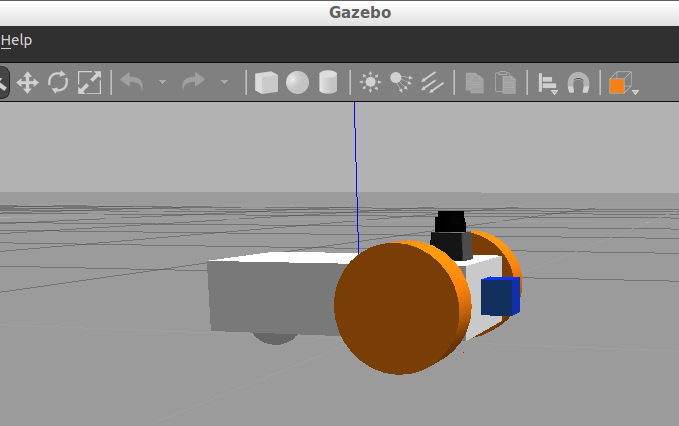
\includegraphics[width=\columnwidth]{images/rover_version_2_gazebo.png}
      \caption{Second version of custom rover. Screenshot in Gazebo.}
      \label{fig:rover_2_design}
\end{figure}
\begin{figure}[thpb]
      \centering
      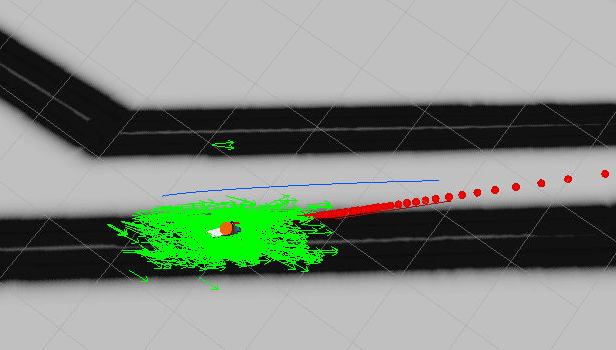
\includegraphics[width=\columnwidth]{images/rover_version_2_toppled_rviz.png}
      \caption{Second version of custom rover toppled over. Screenshot in RViz with global cost map in background.}
      \label{fig:rover_2_toppled}
\end{figure}

In the third and final iteration, the design and appearance of the body was improved. The chassis is built up from a center part, a wing on the left and right side, and a round fender on each corner. The custom colors orange and sky blue were defined in URDF using the \texttt{material} element. They correspond to \texttt{Gazebo/Orange} and \texttt{Gazebo/SkyBlue} as defined in OGRE format. The colors were used on the wheels and the camera. The wheel layout follows the reference model. It consists of two wheels on the left and right with differential drive and two casters in the front and back center. This wheel layout lets the chassis rotate effortlessly and balances the body so that it does not topple over when it hits an obstacle. The laser scanner is placed on top of the chassis in the front middle. The camera is mounted in the center of the front side of the chassis. The final custom model is depicted in figures \ref{fig:rover_3_gazebo} and \ref{fig:rover_3_rviz}.
\begin{figure}[thpb]
      \centering
      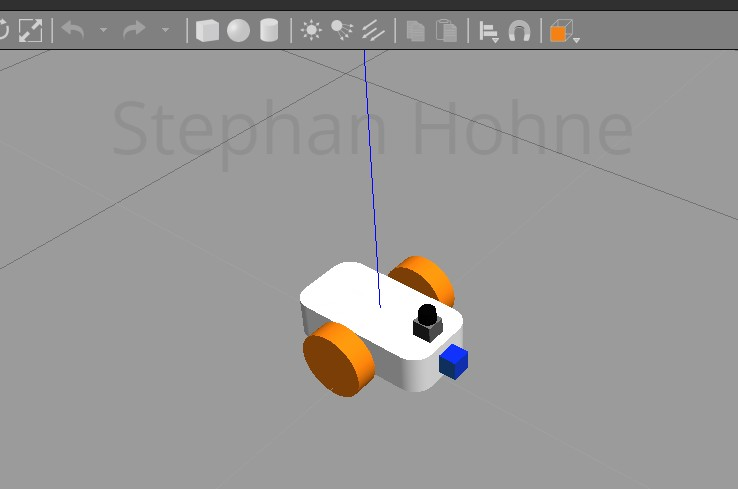
\includegraphics[width=\columnwidth]{images/rover_version_3_gazebo_side.png}
      \caption{Final version of custom rover. Screenshot in Gazebo.}
      \label{fig:rover_3_gazebo}
\end{figure}
\begin{figure}[thpb]
      \centering
      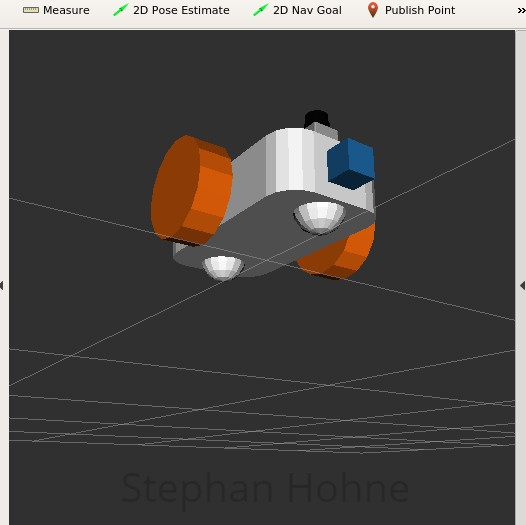
\includegraphics[width=\columnwidth]{images/rover_version_3_rviz_below.png}
      \caption{Final version of custom rover. Screenshot in RViz from below.}
      \label{fig:rover_3_rviz}
\end{figure}

A comparison of the two robot models can be found in table \ref{tab:robot_layout_comparison} and their characteristics are discussed in section \ref{sec:discussion}.
\begin{table}[thpb]
\caption{Characteristic layout parameters for the benchmark model and the final version of the custom rover. The footprint is the corners of the covering rectangle in the $x$-$y$-plane in counterclockwise order.}
\label{tab:robot_layout_comparison}
\begin{center}
\renewcommand{\arraystretch}{1.3}
\begin{tabular}{|l|r|r|}
\hline
Model & \texttt{udacity\_bot} & \texttt{rover} \\
\hline
footprint front left  & $\left(0.225, 0.175\right)$ & $\left(0.235,  0.178 \right)$ \\
footprint rear left   & $\left( -0.2, 0.175\right)$ & $\left(-0.19,  0.178 \right)$ \\
footprint rear right  & $\left( -0.2,-0.175\right)$ & $\left(-0.19, -0.178 \right)$ \\
footprint front right & $\left(0.225,-0.175\right)$ & $\left(0.235, -0.178 \right)$ \\
\hline
chassis length $\times$ width & $0.4 \times 0.2$ & $0.38 \times 0.2$ \\
wheel diameter $\times$ width & $0.2 \times 0.05$  & $0.168 \times 0.056$ \\
wheel separation  & $0.4$  & $0.356$ \\
caster radius & $0.05$ & $0.042$ \\
\hline
\end{tabular}
\end{center}
\end{table}

\section{Background: Navigation Stack}
\label{sec:background_navigation_stack}
This section follows the ROS Wiki tutorial \cite{ros_wiki_nav_stack}. It describes the ROS navigation stack as applied to this project and explains the selection of parameters that was tuned to optimize the localization performance of each robot model. The packages used for navigation are \texttt{amcl} and \texttt{move\_base} with its components \texttt{costmap\_2d} and \texttt{base\_local\_planner}.

The \texttt{amcl} node applies the adaptive Monte Carlo algorithm to perform probabilistic localization and track the pose of the robot within the given map. The \texttt{costmap\_2d} node creates a local and a global cost map that store information about the obstacles in the environment. The \texttt{base\_local\_planner} node calculates global and local trajectories to the goal position. The global cost map is used for creating a long-term plan over the entire map, and the local cost map is used to create a local trajectory. The local planner takes in odometry data to compute velocity commands in order to steer the robot along the local trajectory. An overview of the navigation stack component setup is depicted in figure \ref{fig:overview_navigation_stack}.
\begin{figure*}[thpb]
      \centering
      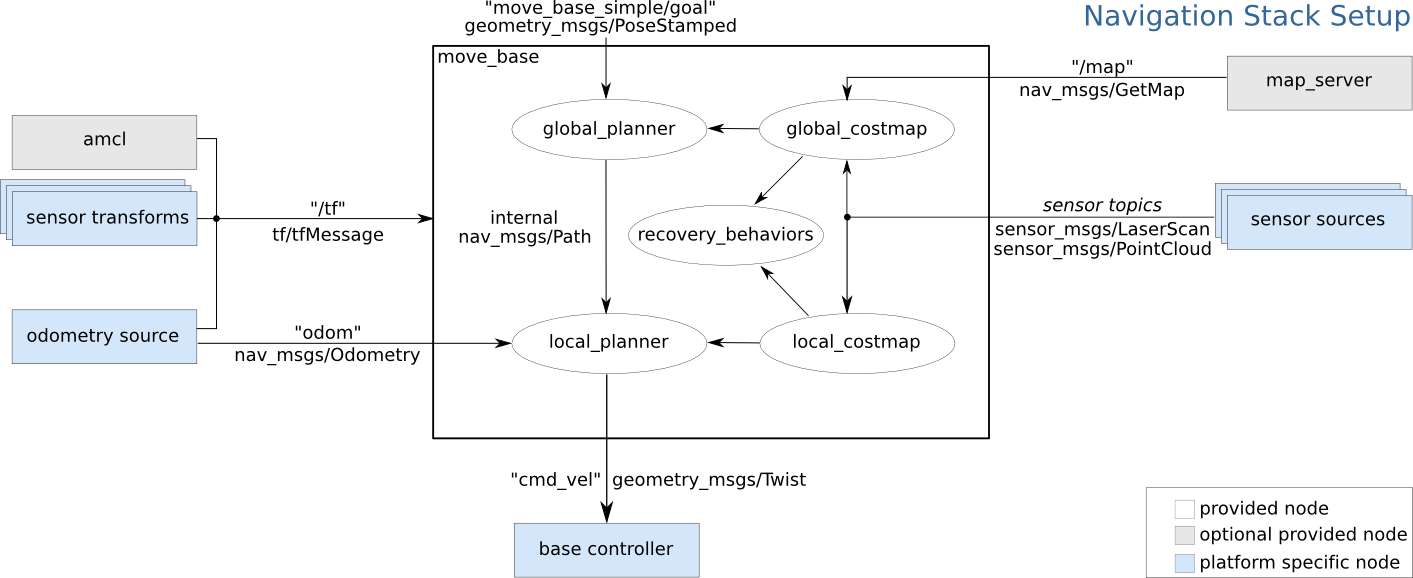
\includegraphics[width=\textwidth]{images/overview_tf.png}
      \caption{Overview of navigation stack component setup. Taken from  \cite{ros_wiki_nav_stack}.}
      \label{fig:overview_navigation_stack}
\end{figure*}

\subsection{Adaptive Monte Carlo Localization}
The \texttt{amcl} package implements the adaptive Monte Carlo localization algorithm \cite{ros_wiki_amcl}. With this approach to localization, a particle filter is used to track the pose of a robot within a given map.

The \texttt{amcl} node subscribes to the topics \texttt{scan} for receiving laser scans, \texttt{tf} for receiving frame transforms, \texttt{initialpose} for initializing the particle cloud, and \texttt{map} for retrieving the map from the server. It publishes the estimated pose and covariance of the robot to \texttt{amcl\_pose}, the pose estimates maintained by the filter to \texttt{particlecloud}, and the transform between odometry and map frame to \texttt{tf}. The \texttt{amcl} node provides the service \texttt{global\_localization} to initialize localization by randomly dispersing particles through the free space, and \texttt{request\_nomotion\_update} to manually perform an update of the particle distribution. It calls the service \texttt{static\_map} to retrieve the map.

The parameters for configuring the \texttt{amcl} node are grouped into overall filter, laser model, and odometry model. The following list describes the overall filter parameters.
\begin{description}
\item[\texttt{<min,max>\_particles}] Minimum and maximum allowed number of particles in the cloud. A high number of particles consumes more computing resources during update but also increases confidence of the resulting pose estimate.
\item[\texttt{initial\_pose\_<x,y,a>}] Defines the mean values of the pose $( x,y,\theta )$ used to initialize filter with a Gaussian distribution. Set to $(0,0,0)$ which coincides with the true initial pose of the robot model. Changing this would require to solve the global localization problem, see section \ref{sec:discussion}.
\item[\texttt{transform\_tolerance}] The published transform from odometry to map frame is future dated by the specified amount, to indicate how long the transforms are valid into the future. the default value is $0.1$ seconds.
\end{description}

The following list describes the laser model parameters.
\begin{description}
\item[\texttt{laser\_model\_type}] The type of laser model. In this project, the \texttt{likelihood\_field} model is used.
\item[\texttt{laser\_likelihood\_max\_dist}] Maximum distance for obstacle inflation on the map.
\item[\texttt{laser\_z\_<hit,rand>}] Mixture weight for the hit and random part of the laser model, respectively. The weights should sum up to one.
\end{description}

The following list describes the odometry model parameters.
\begin{description}
\item[\texttt{odom\_model\_type}] The model \texttt{diff-corrected} is used in this project. It uses the \texttt{sample\_motion\_model\_odometry} algorithm from \cite{probabilistic_robotics}. This model uses the alpha noise parameters as defined in \cite{probabilistic_robotics}.
\item[\texttt{odom\_alpha<1,2,3,4>}] Alpha $1$ and $2$ specify the expected noise in the rotation estimate from the rotation and translation component of the robot motion, respectively. Alpha $3$ and $4$ specify the expected noise in the translation estimate from the translation and rotation component of the robot motion, respectively. Higher values make the particle cloud more widespread.
\item[\texttt{<odom,base,global>\_frame\_id}]  The frames for odometry, robot base, and localization publication, respectively. Set to \texttt{odom}, \texttt{robot\_footprint}, \texttt{map}, respectively.
\end{description}

\subsection{Global and Local Cost Map}
The package \texttt{costmap\_2d} is employed to create a global and a local cost map \cite{ros_wiki_costmap_2d}. Each map has a specific configuration, so the parameter values are grouped accordingly.

The \texttt{costmap\_2d} subscribes to the \texttt{footprint} topic in order to receive the robot footprint. It publishes to the \texttt{costmap} and \texttt{costmap\_updates} topic.

The following list describes a selection of the most relevant parameters that are common to both cost maps. The corresponding file is \texttt{costmap\_common\_params.yaml}.
\begin{description}
\item[\texttt{obstacle\_range}] Defines the obstacle detection radius in meters. The robot will only put obstacles in its map that are within the determined radius of the base.
\item[\texttt{raytrace\_range}] Determines the range to which the free space will be ray traced given a sensor reading. The robot will attempt to clear out space in front of it up to the distance set here.
\item[\texttt{footprint}] Determines the footprint of a rectangular robot. The center of the robot is assumed to be at the origin of the reference frame. In the configuration file, the corner points are specified in counterclockwise order.
\item[\texttt{robot\_radius}] Define the radius for a circular robot. Not used since the robots studied in this project have a rectangular footprint.
\item[\texttt{transform\_tolerance}] Sets the maximum delay of transform data updates in seconds. This avoids loosing a link in the \texttt{tf} tree while the keeping an upper limit for the latency in the system.
\item[\texttt{inflation\_radius}] Defines the maximum distance from obstacles at which an obstacle cost is incurred. All trajectories that are farther away from obstacles are treated as having equal cost.
\item[\texttt{observation\_sources}] Defines a list of sensors that pass information to the cost map. The laser scan sensor is used in this project.
\item[\texttt{laser\_scan\_sensor}] Defines the properties of the laser scan sensor used in this project. The coordinate frame of the sensor is \texttt{hokuyo}. The \texttt{data\_type} is set to \texttt{LaserScan} message. The \texttt{topic\_name} is set to the laser scan topic that the sensor publishes data on. The \texttt{marking} and \texttt{clearing} parameters are set to true so the sensor will be used to add and clear obstacle information to and from the cost map.
\end{description}

The following list describes a selection of the most relevant parameters for the global cost map. The corresponding file is \texttt{global\_costmap\_params.yaml}.
\begin{description}
\item[\texttt{global\_frame}] Specifies the coordinate frame for the global cost map. Set to the \texttt{map} frame.
\item[\texttt{robot\_base\_frame}] Defines the coordinate frame for the base link of the robot. Set to \texttt{robot\_footprint}.
\item[\texttt{update\_frequency}] Sets the frequency of the map update loop in Hertz.
\item[\texttt{resolution}] The resolution of the map in meters per cell. A higher resolution consumes more computing resources.
\item[\texttt{static\_map}] Determines whether the map should be initialized from a file. Set to true since the \texttt{jackal\_race} map is provided by the map server in this project.
\end{description}

The following list describes a selection of the most relevant parameters for the local cost map. The corresponding file is \texttt{local\_costmap\_params.yaml}.
\begin{description}
\item[\texttt{publish\_frequency}] Specifies the frequency in Hertz for the map to publish visualization information.
\item[\texttt{width}, \texttt{height}] The size of the local map in meters.
\item[\texttt{rolling\_window}] Defines whether the local map will remain centered around the robot.
\end{description}
The parameters \texttt{global\_frame}, \texttt{robot\_base\_frame}, \texttt{update\_frequency}, \texttt{resolution}, and \texttt{static\_map} defined above are used for the local map as well.

\subsection{Base Local Planner}
The package \texttt{base\_local\_planner} provides a controller to drive a mobile robot on a two dimensional plane \cite{ros_wiki_base_local_planner}. The planner creates a trajectory from start to goal location within a given map. The basic idea of trajectory generation is to create a set of sample velocity commands. The current robot state is then projected forward in time to predict what would happen if the sampled commands were applied. Each of the simulated trajectories is then scored using a cost function that evaluates criteria like proximity to the goal, to the global trajectory and obstacles. The highest ranking trajectory is selected and the corresponding velocity commands are sent to the robot.

The base planner node takes in a global path and a cost map to generate velocity commands to send to the mobile base of the robot. It subscribes to the \texttt{odom} topic. The received \texttt{nav\_msgs/Odometry} message gives the local planner the current speed of the robot. The node publishes to \texttt{global\_plan}, \texttt{local\_plan} and \texttt{cost\_cloud} topics in order to enable visualization of the planned local trajectories and cost grid.

The parameter settings for the package are stored in the file \texttt{base\_local\_planner\_params.yaml}. The local planner parameters studied in this project belong to the categories robot configuration, goal tolerance, forward simulation, and trajectory scoring.

For the robot configuration, the limits of the sampling range for acceleration and velocity commands are set with the parameters \texttt{acc\_lim\_<x,y,theta>}, \texttt{max\_vel\_<x,theta>}, and  \texttt{min\_vel\_<x,theta>}, where $(x, y, \theta )$ are the coordinates of the robots pose. The parameter \texttt{holonomic\_robot} specifies whether velocity commands are generated for a holonomic robot. In this case, commands in the $y$-direction can be issued.

The goal tolerance parameters \texttt{yaw\_goal\_tolerance} and \texttt{xy\_goal\_tolerance} define how close the robot must be to the goal position for being considered as having reached it.

The following list describes the forward simulation parameters.
\begin{description}
\item[\texttt{sim\_time}] The amount of time to forward-simulate trajectories.
\item[\texttt{sim\_granularity}] The step size, in meters, to take between points on a given trajectory.
\item[\texttt{angular\_sim\_granularity}] The step size, in radians, to take between angular samples on a given trajectory.
\item[\texttt{vx\_samples}] The number of samples to use when exploring the forward velocity space. Set to the default value of $3$ samples.
\item[\texttt{vtheta\_samples}] The number of samples to use when exploring the angular velocity space. Set to the default value of $20$ samples.
\item[\texttt{controller\_frequency}] The frequency in Hertz at which the base local planner will be called.
\end{description}

Trajectory scoring is achieved using a cost function $C$ which is computed for each sampled trajectory according to the formula
\begin{equation}
\label{eqn:cost_function}
C = \mathtt{pdist\_scale} \, d_p + \mathtt{gdist\_scale} \, d_g + \mathtt{occdist\_scale} \, c_o
\end{equation}
where $d_p$ is the distance from the trajectory endpoint to the path, $d_g$ is the distance from the trajectory endpoint to the local goal, and $c_o$ is the maximum obstacle cost along the trajectory. The coefficients are given by the following weight parameters.
\begin{description}
\item[\texttt{pdist\_scale}] Weights how much the controller should stay close to the given global path.
\item[\texttt{gdist\_scale}] Weights how much the controller should attempt to reach its local goal.
\item[\texttt{occdist\_scale}] Weights how much the controller should attempt to avoid obstacles.
\end{description}
The parameter \texttt{meter\_scoring} specifies whether the distances are expressed in units of meters or cells. 

\section{Simulations: Parameter Tuning}
\label{sec:simulations_parameter_tuning}
The goal of parameter tuning was to find a configuration that optimizes navigation proficiency for each of the two robot models. The initial values for the parameters were either kept at their default or set following suggestions in the ROS Wiki tutorial \cite{ros_wiki_nav_stack}, the project lesson in the classroom, and communication with students. The values for the robot geometry like the footprint were deduced from the URDF description. The initial AMCL configuration is given in table \ref{tab:initial_values_amcl}. The complete set of initial parameters can be found in the repository at the commit \href{https://github.com/S2H-Mobile/RoboND-Localization-Project/tree/9e4680226e74e2f6d12710e168e3d0a65ce26e66}{9e46802}.
\begin{table}[th]
\caption{Initial values for AMCL parameters.}
\label{tab:initial_values_amcl}
\begin{center}
\renewcommand{\arraystretch}{1.3}
\begin{tabular}{|l|l|}
\hline
Parameter & Value \\
\hline
\texttt{transform\_tolerance} & $0.2$ \\
\hline
\texttt{min\_particles} & $20$  \\
\texttt{max\_particles} & $200$ \\
\hline
\texttt{odom\_alpha1} & $0.04$ \\
\texttt{odom\_alpha2} & $0.04$ \\
\texttt{odom\_alpha3} & $0.02$ \\
\texttt{odom\_alpha4} & $0.04$ \\
\hline
\texttt{laser\_likelihood\_max\_dist} & $4.0$ \\
\hline
\texttt{laser\_z\_hit}  & $0.95$ \\
\texttt{laser\_z\_rand} & $0.05$ \\
\hline
\end{tabular}
\end{center}
\end{table}

Starting from the initial configuration, ten AMCL parameters, three base planner parameters, and five cost map parameters were studied. To handle the complexity of tuning $18$ parameters, the approach taken was to set out with exploration experiments that aim at finding values that enable the robot models reach the goal. Each experiment can consist of one or more trial runs of the specified robot model, from the start position at the origin to the goal location as defined by the \texttt{/navigation\_goal} node. Continuing from the results of these experiments, specific parameters were selected for fine tuning and the effect of these parameters on the algorithm performance were studied. All other parameters were kept fixed at the values found in the best performing experimental run.

\subsection{Exploring the Move Base Parameter Space}
\label{sec:move_base_experiments}
For the experimental runs $1$ to $3$, the goal was to explore the parameter space of the move base package in order to find a configuration that lets the robot reach its goal. The experimental runs were performed using the \texttt{udacity\_bot} with the AMCL configuration being fixed at the initial values given in table \ref{tab:initial_values_amcl}. The tuned parameters are shown in table \ref{tab:move_base_experiments}.

\begin{table}[thbp]
\caption{Parameters tuned during move base parameter space exploration experiments. The \texttt{udacity\_bot} was used.}
\label{tab:move_base_experiments}
\begin{center}
\renewcommand{\arraystretch}{1.3}
\begin{tabular}{|l|c|c|}
\hline
Experiment & $1$ & $2$, $3$ \\
\hline
\multicolumn{3}{|l|}{Base local planner} \\
\hline
\texttt{sim\_time}    & $1.0$ & $10.0$  \\
\texttt{pdist\_scale} & $0.6$ &  $0.8$  \\
\texttt{gdist\_scale} & $0.8$ &  $0.6$  \\
\hline
\multicolumn{3}{|l|}{Cost maps} \\
\hline
\texttt{obstacle\_range}   & $2.5$  & $3.0$  \\
\texttt{raytrace\_range}   & $3.0$  & $5.0$  \\
\texttt{inflation\_radius} & $0.55$ & $0.6$  \\
Local map width            & $7.0$  & $6.0$  \\
Local map height           & $7.0$  & $6.0$  \\
\hline 
Screenshot & & \ref{fig:result_experiment_2},  \ref{fig:result_experiment_3}\\
\hline
Repository & & \href{https://github.com/S2H-Mobile/RoboND-Localization-Project/tree/eea80c389c23bcb5522f89777ab40a6292e0076f}{eea80c3}\\
\hline
\end{tabular}
\end{center}
\end{table}

For the \texttt{base\_local\_planner}, the simulation time and the scaling weights from the cost function equation \ref{eqn:cost_function} were tuned, while the parameters for acceleration limits, goal tolerances, simulation granularities, and sample sizes were kept fixed at their default values.

The \texttt{sim\_time} was increased significantly from $1 s$ to $10 s$. The scaling weight \texttt{pdist\_scale} for the path distance $d_p$ was increased from the default $0.6$ to $0.8$, while the \texttt{gdist\_scale} for the local goal distance $d_g$ was decreased from the default $0.8$ to $0.6$. The \texttt{occdist\_scale} parameter was kept fixed at the default value of $0.01$. The achievable velocities were kept fixed at a limit of $\pm 4.0 \, m/s$ for translation in the forward $x$-direction and $\pm 4.0 \, rad/s$ angular velocity around the $z$-axis.

For the cost maps, the obstacle range, the ray trace range, the inflation radius and the size of the local map were tuned. The obstacle range was extended from $2.5$ meters to $3.0$ meters, and the ray trace range was extended from $3.0$ meters to $5.0$ meters. The inflation radius was slightly increased from $0.55$ meters to $0.6$ meters. The size of the local map was reduced from $7.0 \times 7.0$ meters to $6.0 \times 6.0$ meters. The controller frequency was kept fixed at $15.0$ Hertz. The tolerance for transforms between global frame and robot base frame was set to $0.4$ seconds. The publish and update frequencies were set to $15.0$ Hertz for both maps. The resolution was set to $0.02$ as per definition in the map configuration file.

The results of the experiments are stated in section \ref{sec:results} and the parameter tuning is discussed further in section \ref{sec:discussion}.

\begin{figure}[thpb]
      \centering
      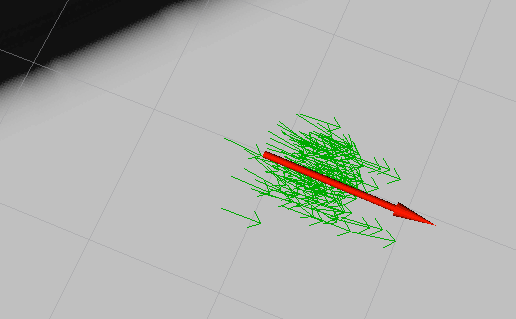
\includegraphics[width=\linewidth]{images/run_2_goal.PNG}
      \caption{Particle cloud at the goal position in run 2 with global costmap in background.}
      \label{fig:result_experiment_2}
\end{figure}

\begin{figure}[thpb]
      \centering
      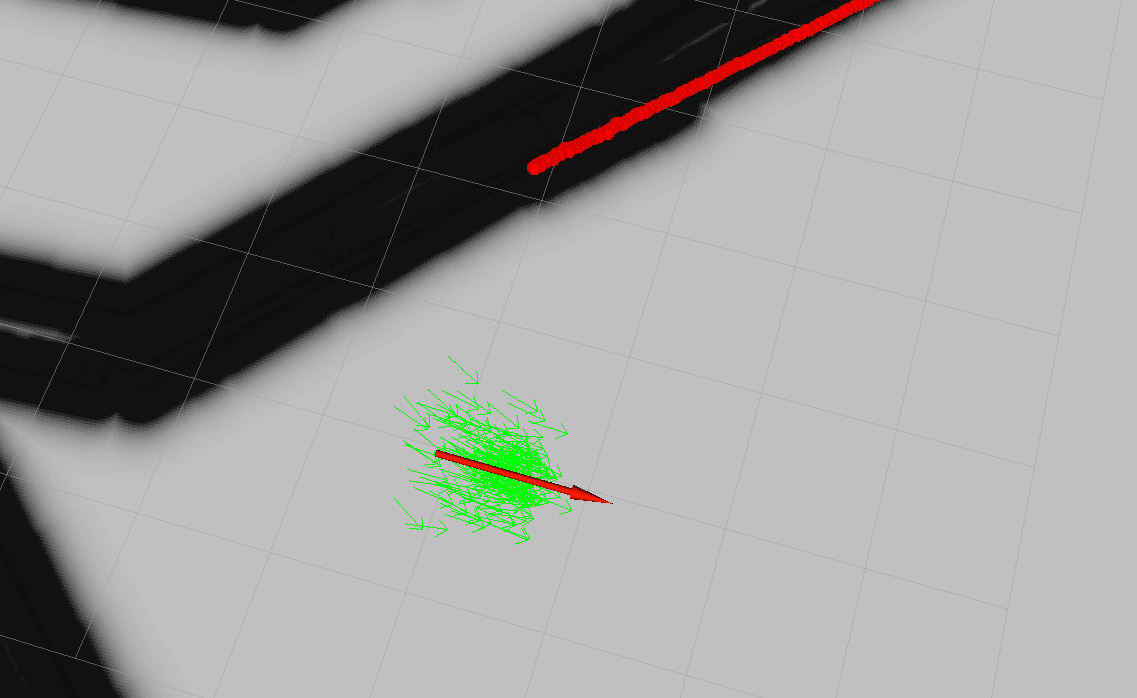
\includegraphics[width=\linewidth]{images/run_3_goal.PNG}
      \caption{Particle cloud at the goal position in run 3 with global costmap in background.}
      \label{fig:result_experiment_3}
\end{figure}

\subsection{Exploring the AMCL Parameter Space}
The experimental runs $4$ to $9$ were dedicated to exploring the parameter space of the AMCL package. The move base parameter values were kept fixed at the settings from run $3$. The tuned parameters are shown in table \ref{tab:amcl_experiments}.

\begin{table}[thbp]
\caption{Parameters tuned during AMCL parameter space exploration experiments.}
\label{tab:amcl_experiments}
\begin{center}
\renewcommand{\arraystretch}{1.3}
\begin{tabular}{|l|c|c|c|c|c|}
\hline
Experiment & $4$ & $5$ & $6$ & $7$ & $8$ \\
\hline
Robot model & \multicolumn{3}{|c|}{\texttt{udacity\_bot}} & \multicolumn{2}{|c|}{\texttt{rover}} \\ 
\hline
Particle number & $100 \ldots 5000$ & \multicolumn{4}{|c|}{$100 \ldots 1000$}\\
\hline
\texttt{odom\_alpha1} & $0.04$  & $0.06$  & \multicolumn{3}{|c|}{$0.05$} \\
\texttt{odom\_alpha2} & $0.04$  & $0.06$  & \multicolumn{3}{|c|}{$0.05$} \\
\texttt{odom\_alpha3} & $0.02$  & $0.01$  & \multicolumn{3}{|c|}{$0.01$} \\
\texttt{odom\_alpha4} & $0.04$  & $0.06$  & \multicolumn{3}{|c|}{$0.05$} \\
\hline
\texttt{laser\_z\_hit}  & \multicolumn{4}{|c|}{$0.95$} & $0.8$ \\
\texttt{laser\_z\_rand} & \multicolumn{4}{|c|}{$0.05$} & $0.2$ \\
\hline
Screenshot  & \ref{fig:result_experiment_4} &  \ref{fig:result_experiment_5} &  \ref{fig:result_experiment_6a}& \ref{fig:result_experiment_7} & \ref{fig:result_experiment_8} \\
\hline
\end{tabular}
\end{center}
\end{table}

In experiment $4$, the particle number range was increased from $20 \ldots 200$ particles to $100 \ldots 5000$ particles. The increase in particle number did not slow down the algorithm noticeably, yet the localization performance was not increased either. The high number of particles introduced a second cluster of particles at the goal location, see image \ref{fig:result_experiment_4}.

In experiment $5$, the maximum particle number was decreased to $1000$ particles The odometry noise parameters were tuned as shown in table \ref{tab:amcl_experiments}. The particle cloud at the goal location was more widespread compared to the previous experiments, see image \ref{fig:result_experiment_5}. The experiments $6$ and $7$ were run with the same parameter values while using the reference and custom model, respectively. The odometry noise parameters set to an intermediate value compared to the previous runs. In experiment $8$, the weights of the laser model were changed. Apart from that, the configuration was the same as in the previous experiments.

The results of the experiments are stated in section \ref{sec:results} and the parameter tuning is discussed further in section \ref{sec:discussion}.

\begin{figure}[thpb]
      \centering
      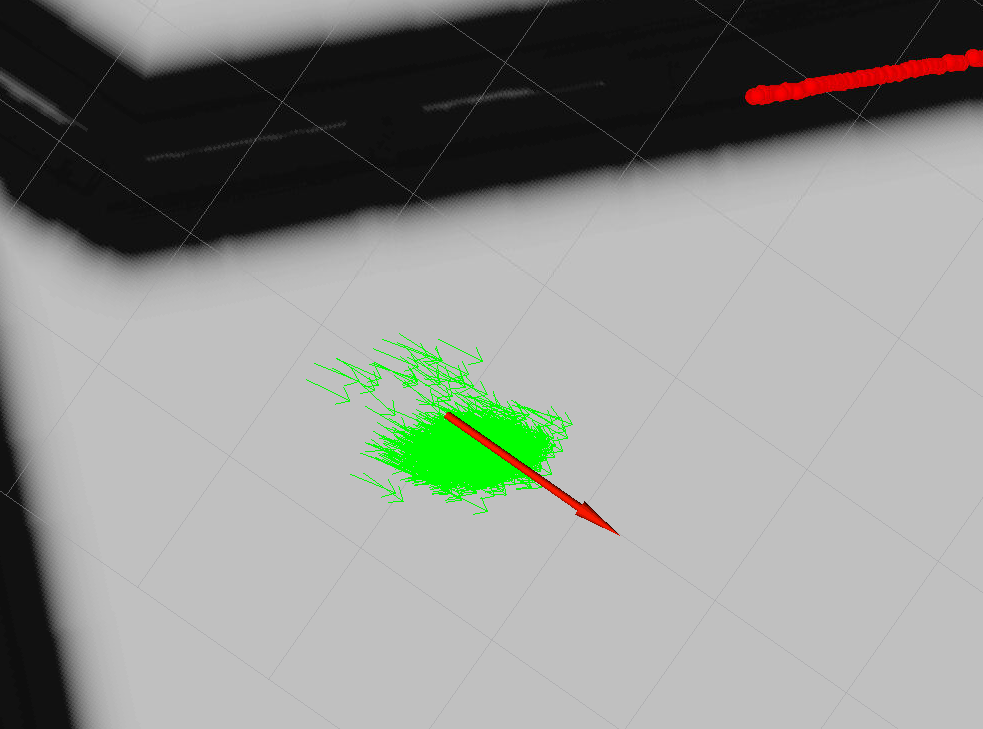
\includegraphics[width=\linewidth]{images/run_4_goal.PNG}
      \caption{Particle cloud at the goal position in run 4 with global cost map in background.}
      \label{fig:result_experiment_4}
\end{figure}

\begin{figure}[thpb]
      \centering
      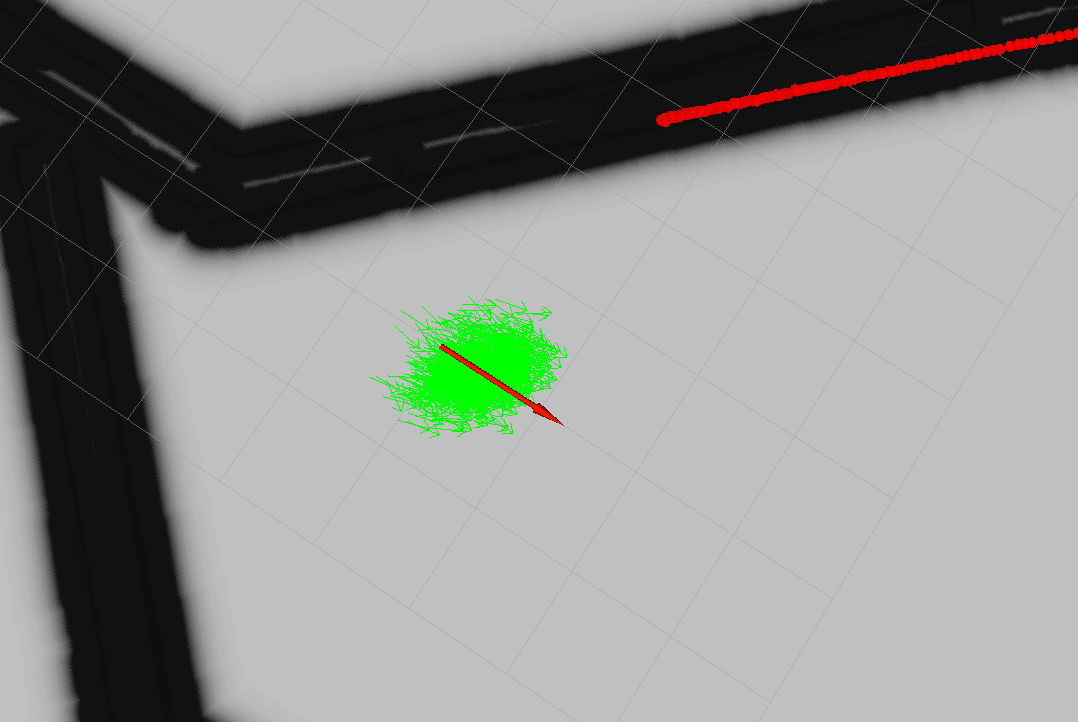
\includegraphics[width=\linewidth]{images/run_5_goal.PNG}
      \caption{Particle cloud at the goal position in run 5 with global cost map in background.}
      \label{fig:result_experiment_5}
\end{figure}

\begin{figure*}[thpb]
      \centering
      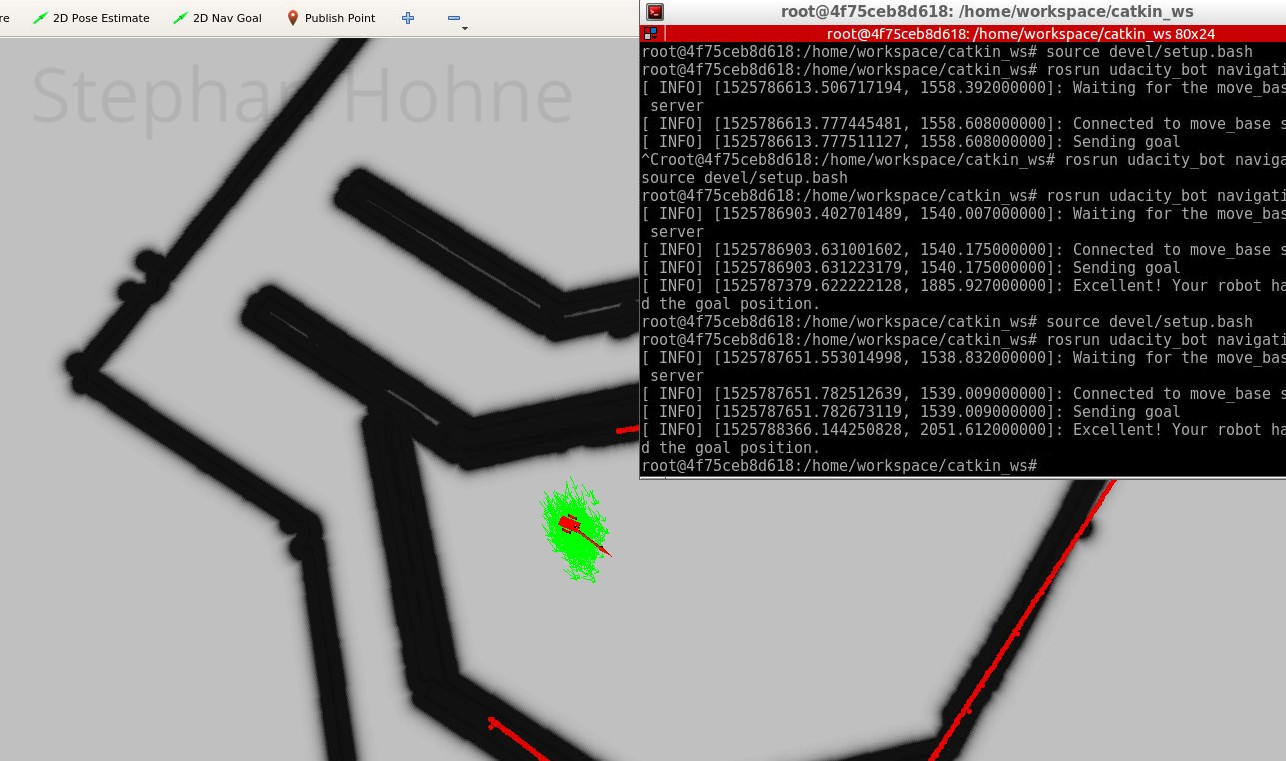
\includegraphics[width=\linewidth]{images/udacity_bot_run_6a_goal_signed.PNG}
      \caption{Benchmark robot model and particle cloud at the goal position in run 6 with global cost map in background.}
      \label{fig:result_experiment_6a}
\end{figure*}

\begin{figure}[thpb]
      \centering
      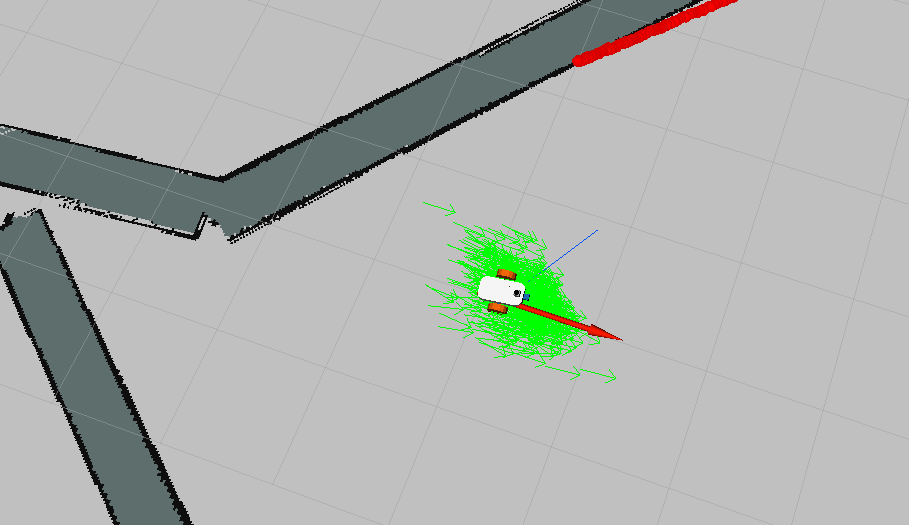
\includegraphics[width=\linewidth]{images/run_7_goal.PNG}
      \caption{Robot and particle cloud at the goal position in run 7 with ground truth map in background.}
      \label{fig:result_experiment_7}
\end{figure}

\begin{figure}[thpb]
      \centering
      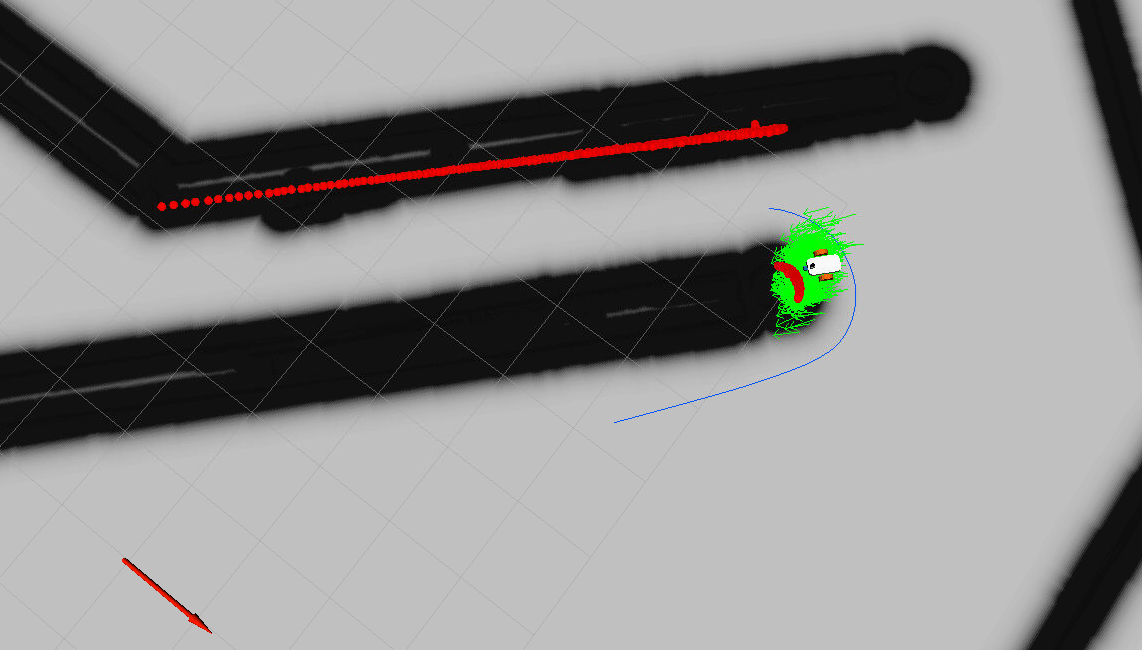
\includegraphics[width=\linewidth]{images/run_8_stuck.PNG}
      \caption{Robot got stuck in run $8$ with global cost map in background.}
      \label{fig:result_experiment_8}
\end{figure}

\subsection{Improving Localization Performance}
The final experiment $9$ was dedicated to improving the localization performance of the navigation stack using the \texttt{rover} model. The experiment aimed at minimizing the drift caused by odometry noise, reducing the spread of the particle cloud at the goal position and letting the local trajectory follow the global path closely without oscillating behavior. The parameters that promised to have the highest impact on these tasks were taken into consideration. The tuned parameters are shown in table \ref{tab:navigation_performance_experiments}.

\begin{table}[thbp]
\caption{Parameters tuned during experiment $9$ for improving localization performance of the navigation stack.}
\label{tab:navigation_performance_experiments}
\begin{center}
\renewcommand{\arraystretch}{1.3}
\begin{tabular}{|l|c|c|c|c|}
\hline
Run & $1$ & $2$ & $3$ & $4$ \\
\hline
\texttt{pdist\_scale} & $2.8$  & \multicolumn{3}{|c|}{$1.8$} \\
\hline
\texttt{odom\_alpha1} & \multicolumn{2}{|c|}{$0.05$} & $0.09$ & $0.02$ \\
\texttt{odom\_alpha2} & \multicolumn{2}{|c|}{$0.05$} & $0.09$ & $0.02$ \\
\texttt{odom\_alpha3} & \multicolumn{2}{|c|}{$0.01$} & $0.05$ & $0.005$\\
\texttt{odom\_alpha4} & \multicolumn{2}{|c|}{$0.05$} & $0.09$ & $0.02$ \\
\hline
Screenshot  & \ref{fig:result_experiment_9-1} & \ref{fig:result_experiment_9-2} & \ref{fig:result_experiment_9-3} & \ref{fig:result_experiment_9-4} \\
\hline
\end{tabular}
\end{center}
\end{table}

For reducing the oscillation behavior of the local trajectory, the scaling weights for the trajectory cost function \ref{eqn:cost_function} were taken under consideration. The \texttt{pdist\_scale} coefficient weights the distance to the global path, so this parameter was selected for tuning with the assumption that increasing its value will reduce oscillations. In the first run, the value was increased significantly to $2.8$, and in the subsequent runs the value was set to an intermediate value of $1.8$. The other weights were left at the values $\mathtt{gdist\_scale}=0.6$ and $\mathtt{occdist\_scale}=0.01$ found in the move base parameter exploration experiments, see section \ref{sec:move_base_experiments}.

In runs 3 and 4 the odometry noise parameters were first tuned up and then tuned down significantly, to estimate their effect on the size of the particle cloud and aiming at reducing the drift of the laser scan relative to the map, see section \ref{sec:results} for the results and section \ref{sec:discussion} for the discussion.

\begin{figure}[thpb]
      \centering
      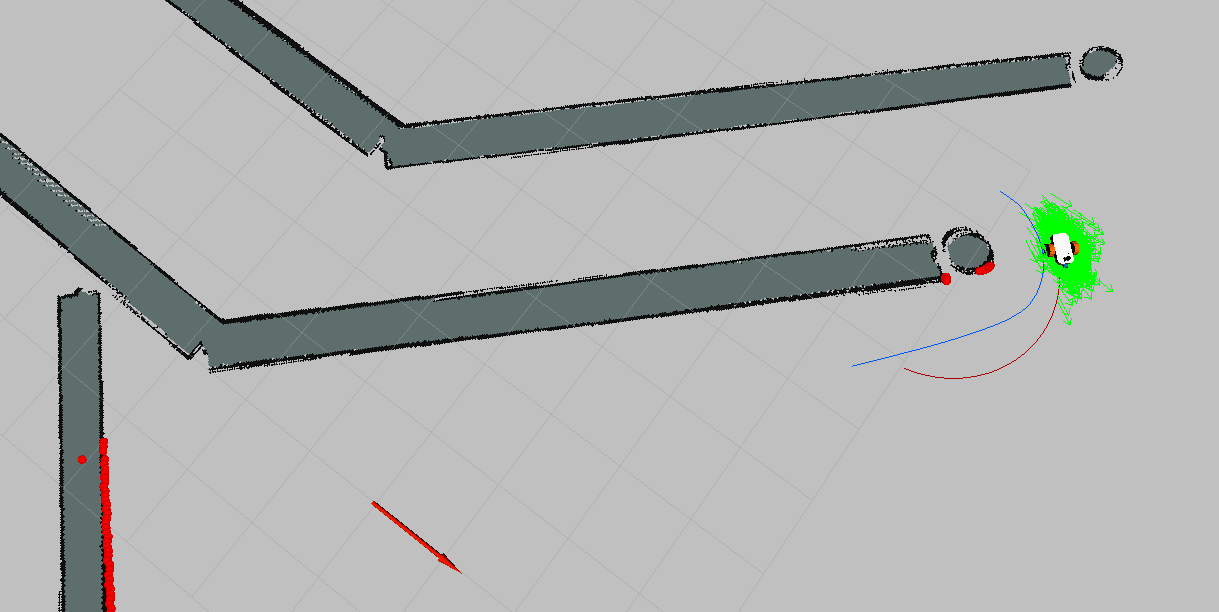
\includegraphics[width=\linewidth]{images/exp_9_run_1.PNG}
      \caption{Custom robot model, particle cloud, local trajectory (red), and global path (blue) during run $1$ in experiment $9$. Screenshot in RViz with ground truth map in background.}
      \label{fig:result_experiment_9-1}
\end{figure}

\begin{figure}[thpb]
      \centering
      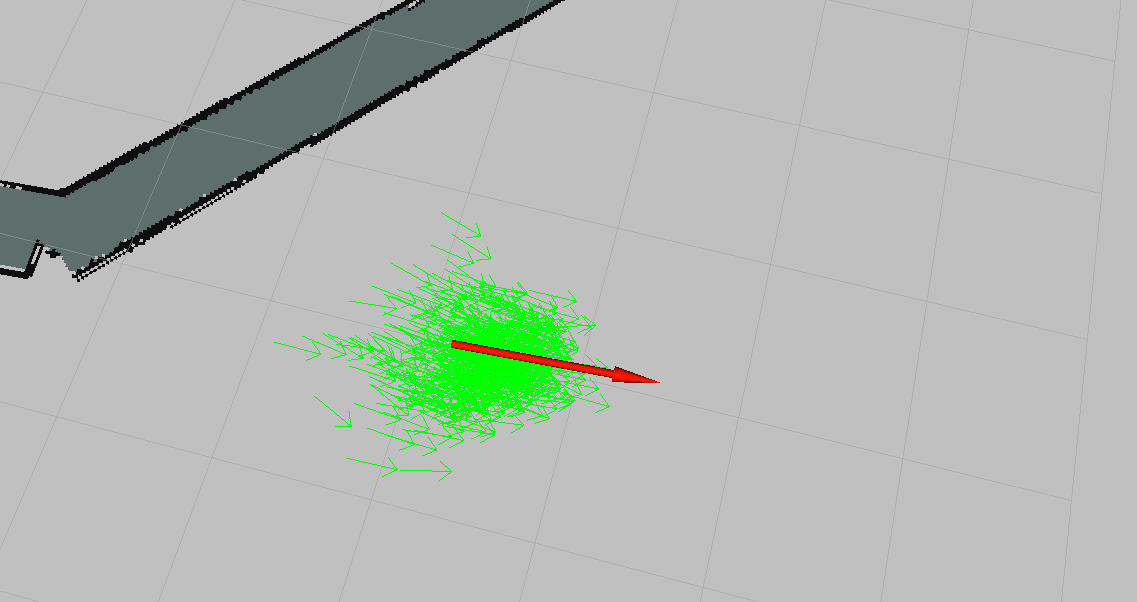
\includegraphics[width=\linewidth]{images/exp_9_run_2_goal.PNG}
      \caption{Particle cloud at goal position in experiment $9$, run $2$. Screenshot in RViz with ground truth map in background.}
      \label{fig:result_experiment_9-2}
\end{figure}

\section{Results}
\label{sec:results}
The navigation proficiency of the robot models was gauged using the visualization information from RViz. The navigation goal was defined by the \texttt{navigation\_goal} node, which also notifies the user whether the robot model has reached the goal successfully.

The first and second version of the custom robot model were not able to navigate to the goal location. The reference model and the final custom model reached the goal location successfully in all experimental runs except 1 and 8.

The \texttt{udacity\_bot} did not reach the goal position in experiment 1, where all the parameters were set to their initial values. The model reached the goal position in experiments 2 and 3 after approximately five minutes of simulation time. At the goal, the particle cloud (green arrows) was reasonably well centered around the desired pose (red arrow), see figures \ref{fig:result_experiment_2} and \ref{fig:result_experiment_3}. In experiment  $4$, the robot reached the goal after about five minutes. The particle cloud was centered around the goal with a few outliers, see image \ref{fig:result_experiment_4}. Experiments 5 and 6 showed results similar to experiment 3. From gauging visually the best of those runs was number 6. Image \ref{fig:result_experiment_6a} shows the robot and the particle cloud at the goal position together with the success message from the \texttt{navigation\_goal} node.

The \texttt{rover} model reached the goal in experiment 7, using the configuration that was proven to work with the benchmark model, see image \ref{fig:result_experiment_7}. The \texttt{rover} did not reach the goal in experiment 8 with modified laser model weights, see image \ref{fig:result_experiment_8} and the discussion in section \ref{sec:discussion}. In subsequent runs the laser model parameters were set back to the previously established values.

In experiment 9, the \texttt{rover} reached the goal location in all runs. In the first run with the \texttt{pdist\_scale} significantly increased to $2.8$, the overall navigation performance appeared to improve when compared to the last successful run 7. Yet occasionally the local trajectory displayed erratic behavior and made the robot attempt to run in a circle. Figure \ref{fig:result_experiment_9-1} shows a situation were the local trajectory follows the global path as intended. In the last two runs, the scale was set back to a moderate value of $1.8$. For a discussion of the local trajectory behavior and the scaling weights see section \ref{sec:discussion}.
\begin{figure}[thpb]
	\centering
    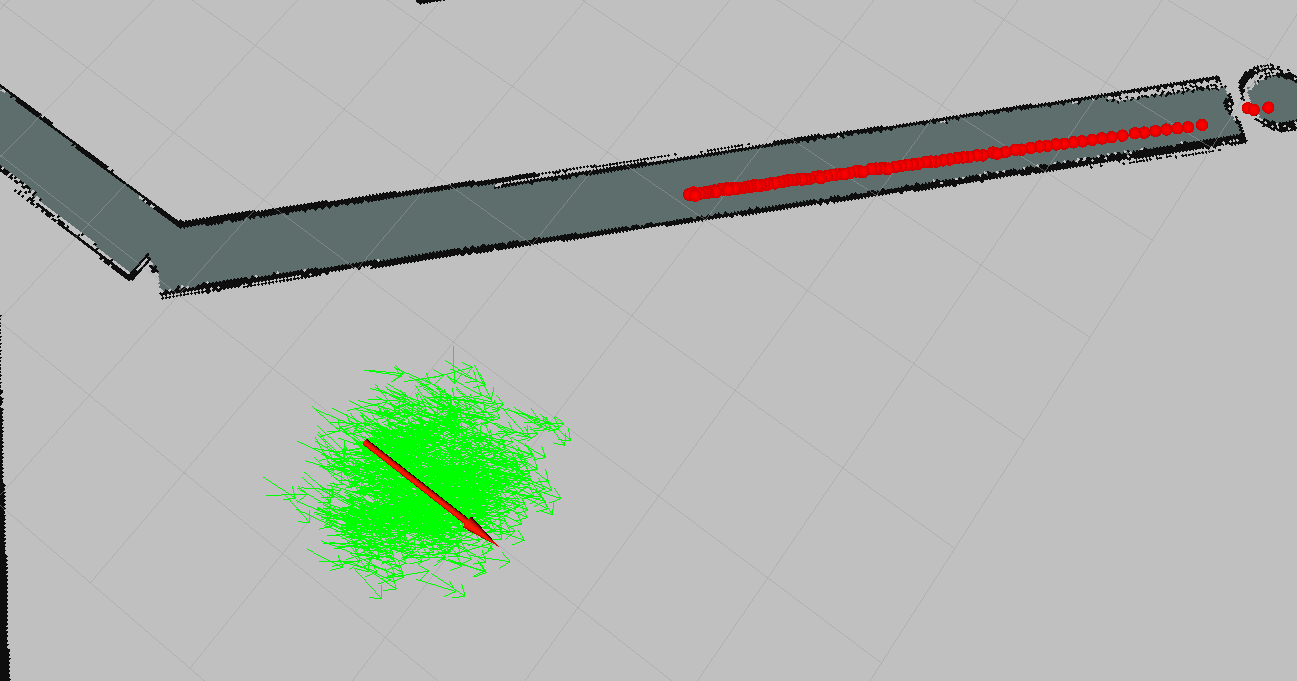
\includegraphics[width=\linewidth]{images/exp9_run3_goal.PNG}
    \caption{Particle cloud at goal position in experiment $9$, run $3$. Screenshot in RViz with ground truth map in background. Laser scan translated relative to the corresponding obstacle.}
    \label{fig:result_experiment_9-3}
\end{figure}

\begin{figure*}[thpb]
	\centering
    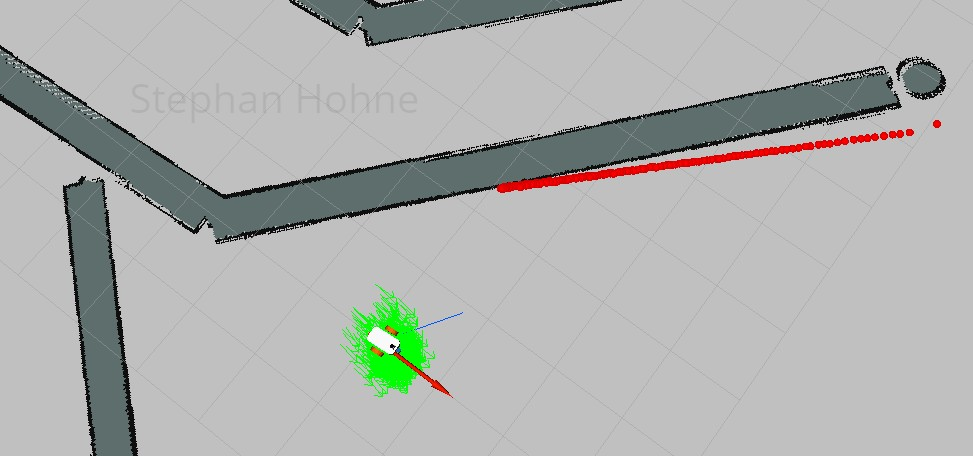
\includegraphics[width=\linewidth]{images/exp9_run4_goal_signed.PNG}
    \caption{Custom robot model and particle cloud at goal position in experiment $9$, run $4$. Screenshot in RViz with ground truth map in background.}
	\label{fig:result_experiment_9-4}
\end{figure*}

The benchmark model and the final custom model performed localization approximately equally well. Both models have a similar layout and the same wheel arrangement. The main physical differences are that the custom rover has a lower center of gravity, wider wheels with reduced diameter, and a more compact body footprint. Consequently both models have similar driving characteristics, with the main difference that the rover is slightly geared down, so that it accelerates a little bit faster and has a slightly slower maximum velocity. Both models have a similar arrangement of the camera and the laser scanner, so both models have essentially the same sensory input. 

Over the experimental runs, the time it took the robot models to reach the goal was reduced from about five minutes to about three minutes, judging from the simulation time in RViz. Except for experiment 9 run 1, the reference model as well as the final version of the \texttt{rover} followed the global path in a reasonable manner.

While the robot models where navigating towards the goal position, it was noticeable in RViz that the laser scan built up a drift. The red laser scan points were rotated and translated with respect to the ground truth map, see images \ref{fig:result_experiment_7}, \ref{fig:result_experiment_9-3}, \ref{fig:result_experiment_9-4}. This effect seemed to be independent of the choice of global frame in RViz, tested with the frames set to \texttt{odom} and \texttt{map}. The third run in experiment $9$ seems to have the smallest drift, see image \ref{fig:result_experiment_9-3}. When looking at runs 3 and 4 in experiment 9 it seems that higher values of the odometry noise alpha parameters reduce the laser scan drift relative to the map, see figure \ref{fig:result_experiment_9-3}, whereas, small values increase it, see figure \ref{fig:result_experiment_9-4}. 

The behavior of the particle cloud was relatively consistent across the experimental runs. The spread of the particle cloud reduced after a few update  iterations. In experimental run 4, a small off-location cluster formed and followed the main cluster, see image \ref{fig:result_experiment_4} and the discussion in section \ref{sec:discussion}.

\section{Discussion}
\label{sec:discussion}
Overall, both the reference and the custom robot model showed a good performance when navigating to the goal location. They reached the goal within a reasonable time and good precision. One way to increase the accuracy of the final robot pose is to reduce the goal tolerance parameters further.

The simulations were performed on the GPU enabled virtual machine. Due to the available compute resources, the simulation speed was good at all tested parameter settings. In a more resource constrained environment, additional effort has to be put in optimizing the map size and forward planning horizon, for example by reducing the \texttt{sim\_time} for the local planner, or particle number for AMCL.

The challenge in exploring the $18$-dimensional space spanned by the tuned parameters is that there might be correlations between different parameters, such that the effect of a single parameter on the navigation performance might depend on the configuration of the other parameters. Nonetheless, the effect of some parameters could be observed. For instance, higher values of the odometry noise parameters seem to reduce the drift, see experiment 9 and figures \ref{fig:result_experiment_9-3}, \ref{fig:result_experiment_9-4}.

In experiment 9 run 1 with the \texttt{pdist\_scale} set to $2.8$, the local trajectory displayed an erratic behavior. At points in the simulations when the global path was U-shaped, the local trajectory was circular which made the robot to either attempt a sharp turn back or to stop abruptly. The behavior improved when the \texttt{pdist\_scale} was lowered to $1.8$. During experiment 9 it was observed that the trajectory scaling weights in the cost function \ref{eqn:cost_function} have a strong impact on the navigation fidelity. Since they have only little effect on algorithm running time by definition, it seems promising to tune them in compute resource constrained environments.

%One way of simulating the global localization problem in the given environment is to set the AMCL parameters \texttt{initial\_pose\_<x,y,a>} to a location away from the origin $(0,0,0)$, so that the particle cloud is not centered at the robots location when the simulation starts.

The AMCL configuration can be modified to be able to solve the relocalization or kidnapped robot problem. To accommodate for a lost pose, the parameters \texttt{recovery\_alpha\_fast} and  \texttt{recovery\_alpha\_slow} have to be enabled and tuned. They control the introduction of random poses in the cloud in situations where the measurement likelihood drops when laser scans come in from the teleported location. This enables the particle cloud to regenerate at the new location \cite{ros_wiki_amcl}.

The methods studied here can be applied to all situations where the pose of a robot needs to be estimated within a 2D world. The key requirement is the availability of an up to date and high-resolution map of the environment. One important application is the navigation of delivery robots in warehouses \cite{warehousing}.

\section{Future Work}
\label{sec:future_work}
The main project goal of enabling two robot models to navigate through a maze to a goal location has been accomplished. The custom robot model can be further optimized to increase navigation proficiency as follows.
\begin{itemize}
\item Make the chassis more compact to ease acceleration and improve driving characteristics. 
\item Optimize center of gravity to avoid toppling over.
\item Determine the actual velocity limits of the models, and set the precise values in the base local planner.
\item Develop a four-wheel design. Be aware of the increased complexity, since it can't turn in place.
\item Develop a holonomic wheel design, so that velocity commands perpendicular to forward direction can be issued.
\item Sensor equipment and placement. Place the laser in the center of the chassis. Try out an additional backward camera on the four-wheel design.
\end{itemize}
The navigation stack configuration can be further optimized to increase navigation proficiency as follows.
\begin{itemize}
\item Study the effect of the laser model parameters on navigation proficiency. The starting point is experiment 8, where the robot model did not reach the goal.
\item Do more experiments to balance all three scaling weights in the cost function \ref{eqn:cost_function}. The starting point is experiment 8, where only \texttt{pdist\_scale} was tuned.
\end{itemize}

It is left to future work to deploy the navigation stack developed here to actual hardware. A basic physical rover would consist of a chassis with differential drive, a compute module running ROS like the Jetson TX\ 2, a camera, and a laser scanner or ultrasound sensor. The main open question is whether the Jetson TX\ 2 has sufficient compute resources to run the navigation stack fast.

\bibliographystyle{ieeetr}
\begin{thebibliography}{8}

\bibitem{principles_of_robot_motion}
Howie Choset, Kevin M.\ Lynch, Seth Hutchinson, George Kantor, Wolfram Burgard, Lydia E.\ Kavraki and Sebastian Thrun, \textit{Principles of Robot Motion}, The MIT Press, 2005

\bibitem{probabilistic_robotics}
Sebastian Thrun, Wolfram Burgard and Dieter Fox, \textit{Probabilistic Robotics}, The MIT Press, 2005

\bibitem{monte_carlo_for_mobile_robots}
F.\ Dellaert, D.\ Fox, W.\ Burgard, S.\ Thrun, \textit{Monte Carlo localization for mobile robots}, Proceedings 1999 IEEE International Conference on Robotics and Automation (Cat. No.99CH36288C), Detroit, MI, 1999, pp. 1322-1328 vol.2.

\bibitem{ros_wiki_nav_stack}
\textit{Setup and Configuration of the Navigation Stack on a Robot},
\href{http://wiki.ros.org/navigation/Tutorials/RobotSetup/}{ROS Wiki Tutorial}, Open Source Robotics Foundation

\bibitem{ros_wiki_base_local_planner}
\textit{Package Summary Base Local Planner},
\href{http://wiki.ros.org/base_local_planner}{ROS Wiki}, Open Source Robotics Foundation

\bibitem{ros_wiki_costmap_2d}
\textit{Package Summary Costmap 2D},
\href{http://wiki.ros.org/costmap_2d}{ROS Wiki}, Open Source Robotics Foundation

\bibitem{ros_wiki_amcl}
\textit{Package Summary AMCL},
\href{http://wiki.ros.org/amcl}{ROS Wiki}, Open Source Robotics Foundation

\bibitem{warehousing}
Goran Vasiljevi´c, Damjan Mikli´c, Ivica Draganjac, Zdenko Kovaˇci´c, Paolo Lista, \textit{High-accuracy vehicle localization for autonomous
warehousing}, Preprint submitted to Robotics and Computer-Integrated Manufacturing, 2016, \href{https://bib.irb.hr/datoteka/816062.warehousing_localization.pdf}{online link}
\end{thebibliography}
\end{document}